\documentclass[12pt,a4paper]{article}
\linespread{1.1}
\usepackage[utf8x]{inputenc}
\usepackage{ucs}
\usepackage{amsmath}
\usepackage{bm}
\usepackage{amsfonts}
\usepackage{amssymb}
\usepackage{graphicx}
\usepackage{wrapfig}
\usepackage{lipsum}
\usepackage[hidelinks]{hyperref}
\usepackage{indentfirst}
\usepackage[margin=1cm]{caption}
\usepackage{siunitx}

\usepackage[superscript, nomove]{cite}

\makeatletter
\renewcommand{\@citess}[1]{\textsuperscript{[#1]}}
\makeatother

\newcommand{\citein}[1]{[\citen{#1}]}

\usepackage[left=2.2cm, right=2.2cm, top=2.2cm, bottom=2.2cm]{geometry}

\usepackage[svgnames]{xcolor}
\definecolor{blue}{RGB}{13,71,161}


\author{Jakub Bartosz Dranczewski}
\title{Designing, Simulating, and Optimising Nanoantennas that utilise Nonlinear Effects}
\date{}
\begin{document}

\begin{titlepage}
	\begin{center}
		\vspace*{1cm}
		
		\Huge
		\textbf{Designing, Simulating, and Optimising Nanoantennas that utilise Nonlinear Effects}
		
		\Large
		A literature review
		
		\vspace{1.2cm}
		\large
		Project: EXSS-Sapienza-1\\
		Project partner: Taran Attavar\\
		Supervisor: Riccardo Sapienza\\
		Assessor: Cynthia Vidal
		
		\vspace{1.5cm}
		
		\textbf{Jakub Bartosz Dranczewski}
		
		\vfill
		
		
\includegraphics[width=0.4\textwidth]{img/Imperial-logo.pdf}
		
		\vspace{0.4cm}
		
		
		Word count: NaN (max is 2500)
		
	\end{center}
\end{titlepage}

\begin{abstract}
\lipsum[9]

\end{abstract}

\section{Introduction}
The goal of our project is to investigate, both experimentally and computationally, the applicability and efficiency of different nanoantenna designs for enhancing nonlinear optical effects at the nanoscale. Light manipulation using the nonlinear response of materials has existing and promising future applications in a number of areas, including frequency control for laser light, optical communications, spectroscopy, data storage, and sensing\cite{garmireNonlinearOpticsDaily2013a}. Nonlinear effects often require large interaction volumes and high laser powers to occur, and nanoantennas are one of the proposed ways to alleviate this and bring nonlinear optics to small-scale applications.

\section{Nonlinear optics}
\label{section:nonlinear-optics}
When considering the propagation of light in matter, it is often assumed that the response of the material is linear\cite{jacksonClassicalElectrodynamics1999}, giving a simple expression for the polarisation:
\begin{equation}
	\label{eq:linear-polarisation}
	\bm{P}=\epsilon_0\chi\bm{E},
\end{equation}
with $\epsilon_0$ being the permittivity of free space, and $\bm{E}$ the electric field. As outlined in \citein{boydNonlinearOptics2008}, this expression can be generalised to include terms that only gain significance at higher field magnitudes, and can be thought to correspond to potentials for the electrons in the material deviating from the simple harmonic approximation:
\begin{align}
	\label{eq:nonlinear-polarisation}
	\bm{P}&=\epsilon_0(\chi^{(1)}\bm{E}+\chi^{(2)}\bm{E}^2+\chi^{(3)}\bm{E}^3+...)\\
	&=\bm{P}^{(1)}+\bm{P}^{(2)}+\bm{P}^{(3)}+...,
\end{align}
where $\chi^{(n)}$ is known as the $n^{th}$ order nonlinear susceptibility, and is in general a tensor.

Now if we allow $\bm{E}$ to vary in time we will also get time variation in $\bm{P}$, and that movement of charges drives a further electric field oscillation. One can then see how the nonlinear terms in \eqref{eq:nonlinear-polarisation} lead to additional frequency components in this new oscillation. For a simple example adapted from \citein{boydNonlinearOptics2008}, we can take $\bm{E}(t)=\bm{E}_0\cos(\omega t)$ and look at the second order polarisation:
\begin{equation}
	\label{eq:example-polarisation}
	\bm{P}^{(2)}=\frac{\epsilon_0\chi^{(2)}}{2}\bm{E}_0^2\left(1+\cos(2\omega t)\right).
\end{equation}
This then drives an electromagnetic wave (the \emph{signal}) at angular frequency $2\omega$, compared to $\omega$ for the incoming (\emph{pump}) wave. The process is known as second harmonic generation (SHG).

Other basic nonlinear processes of note include third harmonic generation (THG), sum and difference frequency generation ($\omega'=\omega_1\pm\omega_2$), changes to the refractive index (a third order process), and others\cite{boydNonlinearOptics2008}.

%TODO this section may want to be shortened, it is quite long - and we basically throw phase matching out the window once we arrive in nanoantenna land.
The \emph{phase matching} parameter, $\Delta k = k'-k$ is crucial in designing most nonlinear processes that involve a change in frequency\cite{boydNonlinearOptics2008}. As both the pump (wavevector $k$) and signal ($k'$) fields interact with the same electric dipoles, the best conditions for coupling between them is when they are in phase such that they don't interfere destructively. While achieving $\Delta k=0$ is possible through anomalous dispersion, it is more feasible to do this by utilising birefringence\cite{raoNonlinearFrequencyConversion2004}. This is only possible for some materials, but if done correctly it can lead to quadratic dependence of the signal density on the interaction distance. On the other hand, if $\Delta k\neq 0$, choosing the wrong sample length can lead to a total loss of signal.

\section{Material considerations}
There is a number of factors to consider when choosing a material for nonlinear interactions. The nonlinear susceptibility is different for different materials\cite{burnsThirdHarmonicGenerationAbsorbing1971}, and can also vary spectrally\cite{carnemollaDegenerateOpticalNonlinear2018a}. Second order effects also demand an asymmetry of potential, which cannot be present in centrosymmetric materials, and as such no bulk second order effects will be present in them, only surface ones\cite{boydNonlinearOptics2008}.

While metals can be used as a medium for nonlinear effects, the currents appearing in them encounter resistance, which leads to losses. This is one of the reasons for a shift towards  utilising dielectric materials, where we have displacement currents instead\cite{krasnokAlldielectricOpticalNanoantennas2012,vandegroepDesigningDielectricResonators2013}, and can choose samples that have a large refractive index (needed for field confinement) and low absorption, preferably both at the pump and signal frequencies.

A useful property that some materials, like Indium Tin Oxide (ITO), exhibit is epsilon-near-zero (ENZ). In these materials the real part of the relative permittivity goes to zero for electromagnetic waves at a given wavelength ($\lambda_{ENZ}$). This has interesting effects on light propagation, but importantly for us it can lead to an enhancement of $\chi^{(3)}$, and greatly increased field confinement\cite{reshefNonlinearOpticalEffects2019}. This can give significant enhancement of nonlinear effects. %TODO provide a number.

\section{Nanoantennas}
For some applications, especially in the field of optical devices, %TODO cite
we may want to couple far-field radiation into the near-field by concentrating it in subwavelength nanostructures. This can be achieved using nanoantennas, which are small formations of metal or dielectric usually designed to have resonances that capture and enhance the field inside\cite{krasnokAlldielectricOpticalNanoantennas2012}.

Simple antenna shapes (for example cylinders) can be considered in terms of basic resonances similar to the ones described by the Lorenz-Mie theory for spheres\cite{sainNonlinearOpticsAlldielectric2019}. Fig.~\ref{fig:modes2} shows a set of these resonances classified as electric, magnetic, and toroidal. Note that metallic antennas only produce significant resonances of the electric type, and mostly through surface effects\cite{kuznetsovOpticallyResonantDielectric2016} -- this is due to field suppression inside a metal. The ability to support both electric and magnetic modes is thus another advantage of dielectrics.
\begin{figure}[h]
	\centering
	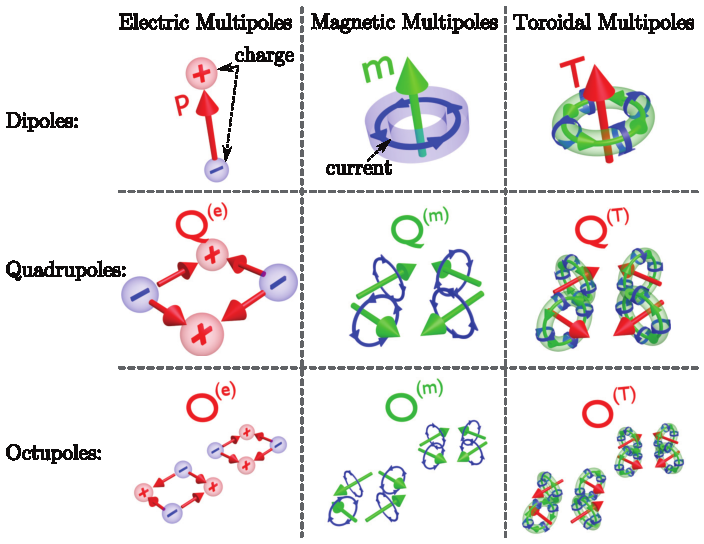
\includegraphics[width=5in]{img/modes2}
	\caption{The three lowest orders of electric, magnetic, and toroidal modes. Superpositions of these can be excited in nanoantennas. Adapted from \citein{savinovToroidalDipolarExcitation2014}.}
	\label{fig:modes2}
\end{figure}

In practice these resonances can spectrally overlap and combine to form modes observable in the antenna's scattering spectrum -- their far-field response. A notable example of this is the anapole mode, for which the toroidal and electric dipoles destructively interfere in the far-field, creating an \emph{dark} mode with low scattering\cite{grinblatEnhancedThirdHarmonic2016}. Mode superpositions can also be utilised to direct the antennas output through far-field interference.

While this discussion focused on simple antenna shapes, more complex arrangements can be used to achieve various output goals. For example, \citein{krasnokAlldielectricOpticalNanoantennas2012} demonstrates how a set of $\sim$\SI{1}{\micro\meter} diameter silicon spheres laid out in analogy to the Yagi-Uda radio-frequency antenna design can result in output beam-widths as low as \SI{40}{\degree}.

\section{Enhancing nonlinear effects with nanoantennas}
An important advantage of nanoantennas as a nonlinear medium is that their subwavelength scale relaxes the phase matching condition\cite{sainNonlinearOpticsAlldielectric2019}, making the design easier and allowing for simplified use of non-birefringent materials. The decreased size results in a disadvantage for nonlinear interactions -- the smaller interaction volume. Beyond the intuitive diminishing of signal when we reduce the amount of material emitting it, there is also the significant dependence of the signal intensity on the interaction length, which can be quadratic in some cases (as seen in Section~\ref{section:nonlinear-optics}). To make up for this we rely on the field enhancing properties of nanoantennas.

Research to mention:

\cite{koshelevSubwavelengthDielectricResonators2020} ("Subwavelength dielectric resonator for nonlinear..."),
Probably keep till last, as an illustration of the importance of good mode selection - this approach results in much greater efficiencies than the other ones.

\cite{grinblatEnhancedThirdHarmonic2016} ("Enhanced...") - the anapole one
Good throwback to the anapole mode, talk about correlation between field confinement and the radiating out (scattering valley - energy peak). They provide an absolute efficiency, and a comparison to a reference film, \emph{and} a different mode. Very nice!

\cite{cambiassoBridgingGapDielectric2017} ("Bridging...") - the one with an increased surface area
Talk about SHG as a surface effect, and the increased surface area as a factor. Same material for ND and substrate, mode chosen such that field enhanced near surface (x30), multiply by the surface area, x1350 increase compared to just bulk! Large overall efficiency, they claim the largest.

\section{Predicting and optimising the nonlinear signal of an antenna}
Small derivation from Lorenz reciprocity. Explain why this method is good. Finite-difference time domain stuff. Mention Lumerical.

Talk about the steps from \citein{koshelevSubwavelengthDielectricResonators2020} (again?). Experimental methodology, computing. Combining materials. This section seems a bit useless...

\section{Conclusion}
You wish you were concluding\cite{aluTheoryModelingFeatures2013}.

\bibliographystyle{myIEEEtran}
% argument is your BibTeX string definitions and bibliography database(s)
\bibliography{IEEEabrv,bib.bib}

\end{document}
